\section{Background} % Numbered section

%------------------------------------------------
\subsection{Why Machine Learning?}
% why ML?
One of the most common reasons PdM methods fail is a lack of continuous improvement and a lack of repeatability \cite{whypdmfails}.
Additionally, equipment monitoring is a time consuming process, requires experts to identify failure patterns, and is expensive.
Machine learning provides an automated approach that requires minimal asset knowledge, is inexpensive, can be trained on many assets, and can be re-trained as operating conditions change.

Machine learning techniques for predictive maintenance were considered not practical, too complex, or too time consuming.
In particular, plant managers did not want to change their existing infrastructure (the software that handles data acquisition and analyzes it) to adopt the technology.
But now Asset Performance Management (APM) software providers are growing and condition based maintenance is at the forefront.
As they team up with cloud based data solutions, it becomes easy for asset operators to implement machine learning in their existing data infrastructures via a simple call to the cloud.
Manufacturers around the world use APM technology from Bentley Systems, a global leader in APM capabilities according to a recent Gartner report \cite{foust_steenstrup_2018}.
The proposed solution will be deployed and maintained using APM software from Bentley Systems.

\subsection{ArcelorMittal Dofasco}
%\subsection{Steel Manufacturing}
% Who is dofasco
ArcelorMittal Dofasco is a steel company located in Hamilton, Ontario.
They use Bentley's APM software and are eager for a machine learning solution to detect the operating conditions of various assets. 
In particular, they have offered a real data set of several industrial level furnace fans located in the Hamilton plant. 
Specifically, the data is composed of several smaller data sets, each representing various hours of operation.
%See the Appendix for full list of variables included.
% Steel mill 
In a steel making plant, called a steel mill, operations run almost 24/7 except when the mill is shut down once a month for repairs and maintenance.
A failure of an asset leading to a shutdown at any other time results in severe costs.
If the operating condition of the asset is known, then operators can determine whether or not it should not be repaired during that scheduled downtime,
thus avoiding costly unexpected failures and the Waddington Effect.


%What is a reheating furnace?
One of the most costly failures occurs when the fans for the reheating furnace fail.
A reheating furnace is used to raise the internal temperature of steel, so that it can be shaped into a final product.
Setting the correct temperature is one of the most essential factors of product quality in the plant.
In fact, the temperature is so high that if the furnace must be inspected, the entire line must be shut down for days to allow the furnace to cool.
%A subject matter expert from ArcelorMittal suggests this could cost millions of dollars in lost production.
A subject matter expert from the steel manufacturer suggests this could cost millions of dollars in lost production.

% about the failure
%One way these furnaces fail is via a failure of the exhaust fans.

%It is therefore critical to steel manufacturers to replace the exhaust fans before a failure occurs.

%------------------------------------------------

\subsection{Self Organizing Maps}

A Self-Organizing Map (SOM) is a type of neural network that is often used as a dimensionality reduction technique as it produces a low dimensional representation of the training samples \cite{kohonen1997exploration}.
A SOM consists of a number of neurons, each represented by a weight vector. 
They are different from other neural networks because they employ competitive learning.
The basic idea behind competitive learning is to have the neurons compete with each other to see who is the most similar to the input vector, `winner takes all' style.
The similarity is usually defined as the Euclidean distance (Eq. \ref{eq:1}) between the input vector and the weight vectors of each neuron.
\begin{equation} \label{eq:1}
    \Vert \boldsymbol{x - w} \Vert_2
\end{equation}

To create a SOM, the size of the map is set to be approximately $5*\sqrt{n}$, where n is number of data points \cite{Tian2014AnomalyDU}. 
The input data is normalized for each variable and the number of neurons are set.
The weights of the closest neurons are updated for each instance in the input data.
Once training is complete, the SOM can be used again to measure the similarity between a test point and the learned mapping.


\begin{figure}[!h]
    \centering
    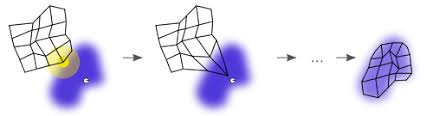
\includegraphics[scale=0.5]{som-learning}
    \caption{A SOM mapping the training data to a two dimensional grid.}
    \label{fig:som-learning}
\end{figure}
